Referring to \cref{fig:spoke-sum}, let $d_\pm$ denote the distance to the focus $f_\pm$ of $\EE$.

Given a point $P=(x,y)\in\EE$ and foci $F_\pm = (\mp c,0)$.
it is elementary to observe
\footnote{See \href{https://en.wikipedia.org/wiki/Ellipse\#Standard_equation}{Ellipse Standard Equation} on Wikipedia, namely: ``The distances from a point $(x,y)$ on the ellipse to the left and right foci are $a+ex$ and $a-ex$''.}
that these distances are linear polynomials
\begin{equation}
\label{eq:foci}
 d_+(P) = a + \frac{cx}{a}, \;\; d_-(P) = a - \frac{cx}{a}
\end{equation}

Thus over $\FF$ their traces are equal to $a$:
\begin{equation}
\label{:dist-focus}
T_N d_+ = T_N d_- = a
\end{equation} 

The curvature $κ(z)$ for a parametrized curve
\begin{equation*}
z\mapsto Z(z) = X(z) + Y(z)\cdot i
\end{equation*}
on a Cartesian Euclidean plane is given\footnote{See \href{https://en.wikipedia.org/wiki/Osculating_circle\#Mathematical_description}{Osculating Circle} on Wikipedia.}
in terms of the first two derivarives $Z',Z''$ 
\begin{equation}
\label{eq:curvature-parametrized}
κ = \frac{Area(Z',Z'')}{|Z'|^3},
\end{equation}

This formula does not depend on the choice of the coordinate
and it is convenient to use derivation with respect to $\log z$
\begin{equation}
W' := z\cdot \frac{\partial W}{\partial z}
\end{equation}
because it preserves the degree: if $Z(z)$ is a Laurent polynomial of degree $d$ then so are $Z'$ and $Z''$,
thus $|Z'|^2 = (Z',Z')$  and $Area(Z',Z'')$ are Laurent polynomials of degree at most $2d$.
Elevating \eqref{eq:curvature-parametrized} to the power $-2/3$ one obtains
\begin{equation}
\label{eq:curvature23-parametrized}
κ^{-2/3} = |Z'|^2 \cdot {Area(Z',Z'')}^{-2/3},
\end{equation}
so for any Laurent polynomial $Z$ the power $κ^{-2/3}$ is a Laurent polynomial
if and only if $Area(Z',Z'')$ is a perfect cube.
For a conic $\deg_z Z = 1$, so $Area(Z',Z'')$ is constant (degree $0$) in $z$.

{\color{orange} Comment this block, but do some experiments first.
For higher degree $d$ Area(Z',Z'') to be a perfect cube seems an unlikely condition.
Explicitly using $z^n \wedge z^m = \frac{z^{n-m} - z^{m-n}}2$
we have for $Z = \sum_{k=-d}^d c(k) z^k$
\begin{equation}
2i \cdot Z' \wedge Z'' = \sum_{n,m=-d}^d c(n)\cdot c(m)^2\cdot \left( z^{n-m}-z^{m-n} \right)
\end{equation}
}

In terms of semi-axes and distances to the foci of the ellipse, the curvature is 
$κ = (a b)\cdot (d_+ d_-)^{-3/2}$,
so the factorization \eqref{eq:curvature23-parametrized} takes the form
\begin{equation}
κ^{-2/3} = \left(d_+ d_-\right) \cdot \left(a b)\right)^{-2/3}.
\end{equation}
Note that $d_\pm$ are degree one by \eqref{eq:foci}.

It follows that $κ^{-2/3}$ is a quadratic polynomial over $\FF$ and for $N>2$ its trace is given by
\begin{equation}
\label{:kappa}
T_N \left(\frac{ab}{κ^2}\right)^\frac{1}{3} = \frac{a^2 + b^2}{2ab}
\end{equation}

\begin{figure}
    \centering
    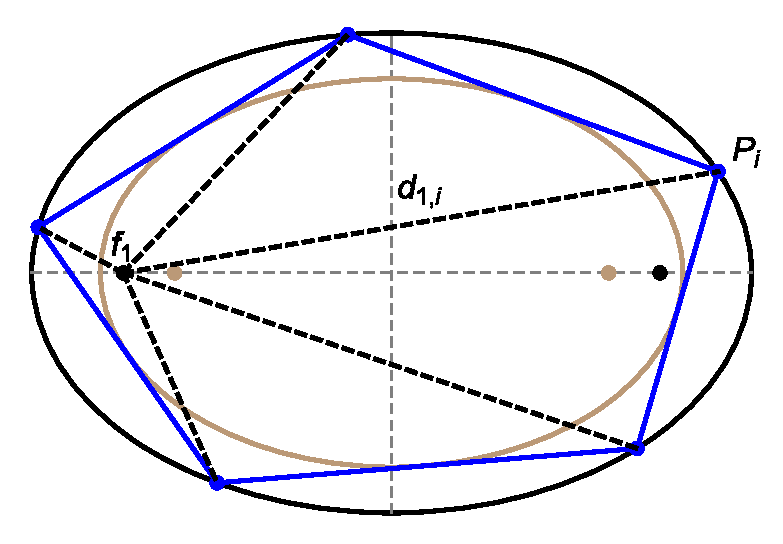
\includegraphics[width=.6\textwidth]{pics/0060_spoke_sum.eps}
    \caption{Over the affinely-regular family, the sum of distances $d_+(P_i)=|P_i-f_+|$ is constant, where $f_+$ is a focus of the outer ellipse.}
    \label{fig:spoke-sum}
\end{figure}
